\section{Busca Sequencial}

\begin{frame}[fragile]\frametitle{Algoritmos de busca}

	\begin{itemize}
        \item Um algoritmo de busca consiste em uma função que identifica se um elemento $x$
        pertence ou não a um conjunto de elementos $S$

        \item A função pode retornar um valor booleano (verdadeiro ou falso), caso o elemento 
        pertença ou não ao conjunto $S$

        \item Outra alternativa é retornar a posição (índice) do elemento no conjunto, caso
        este faça parte do mesmo, ou um valor sentinela, indicando que o elemento não 
        pertence ao conjunto

		\item Caso o conjunto $S$ seja um vetor, o algoritmo de busca mais simples é a busca 
        sequencial, onde todos os elementos do vetor são comparados com o elemento que se deseja 
        encontrar

		\item A ordem de complexidade do algoritmo é $O(N)$, onde $N$ é número de elementos do vetor

		\item Embora existam algoritmos mais eficientes, este algoritmo funciona independentemente
        da ordenação dos elementos do vetor
	\end{itemize}
 
\end{frame}  

\begin{frame}[fragile]{Exemplo de busca sequencial}

    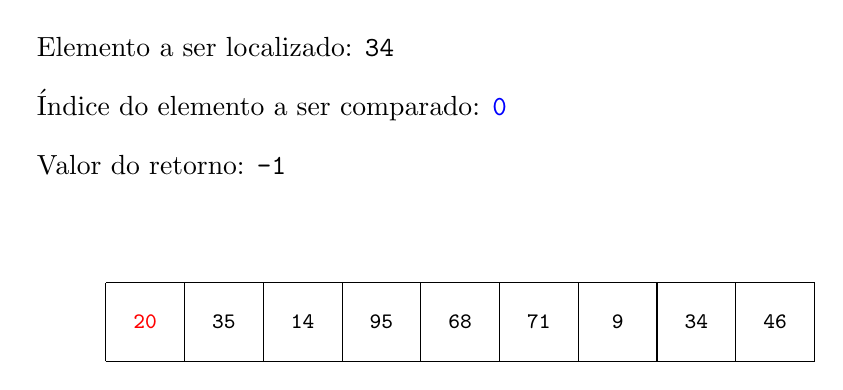
\begin{tikzpicture}
        \node[anchor=west] at (0, 4) {Elemento a ser localizado: \texttt{34}};
        \node[anchor=west] at (0, 3.25) {Índice do elemento a ser comparado: \texttt{\textcolor{blue}{0}}};
        \node[anchor=west] at (0, 2.5) {Valor do retorno: \texttt{-1}};
        \draw (1,0) grid (10,1);

        \node at (1.5,0.5) {\footnotesize \texttt{\textcolor{red}{20}}};
        \node at (2.5,0.5) {\footnotesize \texttt{35}};
        \node at (3.5,0.5) {\footnotesize \texttt{14}};
        \node at (4.5,0.5) {\footnotesize \texttt{95}};
        \node at (5.5,0.5) {\footnotesize \texttt{68}};
        \node at (6.5,0.5) {\footnotesize \texttt{71}};
        \node at (7.5,0.5) {\footnotesize \texttt{9}};
        \node at (8.5,0.5) {\footnotesize \texttt{34}};
        \node at (9.5,0.5) {\footnotesize \texttt{46}};
    \end{tikzpicture}

\end{frame}

\begin{frame}[fragile]{Exemplo de busca sequencial}

    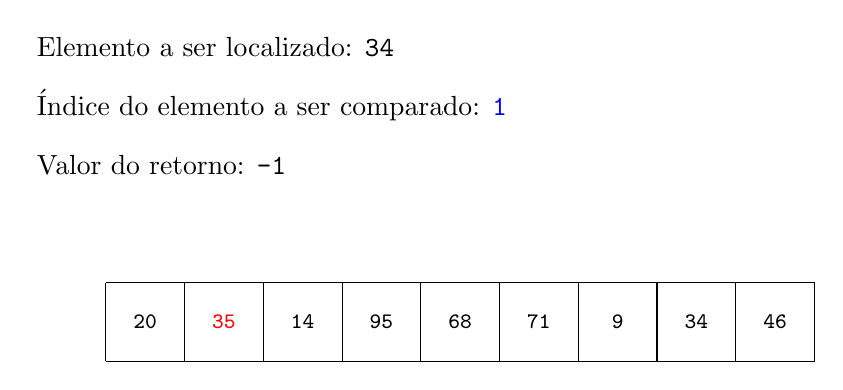
\begin{tikzpicture}
        \node[anchor=west] at (0, 4) {Elemento a ser localizado: \texttt{34}};
        \node[anchor=west] at (0, 3.25) {Índice do elemento a ser comparado: \texttt{\textcolor{blue}{1}}};
        \node[anchor=west] at (0, 2.5) {Valor do retorno: \texttt{-1}};
        \draw (1,0) grid (10,1);

        \node at (1.5,0.5) {\footnotesize \texttt{\textcolor{black}{20}}};
        \node at (2.5,0.5) {\footnotesize \texttt{\textcolor{red}{35}}};
        \node at (3.5,0.5) {\footnotesize \texttt{14}};
        \node at (4.5,0.5) {\footnotesize \texttt{95}};
        \node at (5.5,0.5) {\footnotesize \texttt{68}};
        \node at (6.5,0.5) {\footnotesize \texttt{71}};
        \node at (7.5,0.5) {\footnotesize \texttt{9}};
        \node at (8.5,0.5) {\footnotesize \texttt{34}};
        \node at (9.5,0.5) {\footnotesize \texttt{46}};
    \end{tikzpicture}

\end{frame}

\begin{frame}[fragile]{Exemplo de busca sequencial}

    \begin{tikzpicture}
        \node[anchor=west] at (0, 4) {Elemento a ser localizado: \texttt{34}};
        \node[anchor=west] at (0, 3.25) {Índice do elemento a ser comparado: \texttt{\textcolor{blue}{2}}};
        \node[anchor=west] at (0, 2.5) {Valor do retorno: \texttt{-1}};
        \draw (1,0) grid (10,1);

        \node at (1.5,0.5) {\footnotesize \texttt{\textcolor{black}{20}}};
        \node at (2.5,0.5) {\footnotesize \texttt{\textcolor{black}{35}}};
        \node at (3.5,0.5) {\footnotesize \texttt{\textcolor{red}{14}}};
        \node at (4.5,0.5) {\footnotesize \texttt{95}};
        \node at (5.5,0.5) {\footnotesize \texttt{68}};
        \node at (6.5,0.5) {\footnotesize \texttt{71}};
        \node at (7.5,0.5) {\footnotesize \texttt{9}};
        \node at (8.5,0.5) {\footnotesize \texttt{34}};
        \node at (9.5,0.5) {\footnotesize \texttt{46}};
    \end{tikzpicture}

\end{frame}

\begin{frame}[fragile]{Exemplo de busca sequencial}

    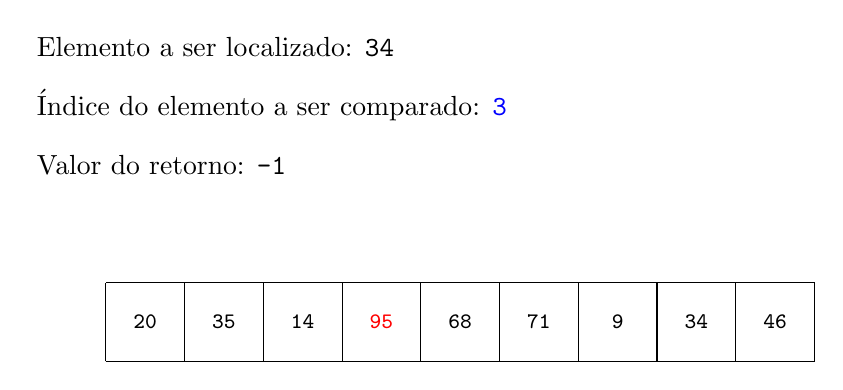
\begin{tikzpicture}
        \node[anchor=west] at (0, 4) {Elemento a ser localizado: \texttt{34}};
        \node[anchor=west] at (0, 3.25) {Índice do elemento a ser comparado: \texttt{\textcolor{blue}{3}}};
        \node[anchor=west] at (0, 2.5) {Valor do retorno: \texttt{-1}};
        \draw (1,0) grid (10,1);

        \node at (1.5,0.5) {\footnotesize \texttt{\textcolor{black}{20}}};
        \node at (2.5,0.5) {\footnotesize \texttt{\textcolor{black}{35}}};
        \node at (3.5,0.5) {\footnotesize \texttt{\textcolor{black}{14}}};
        \node at (4.5,0.5) {\footnotesize \texttt{\textcolor{red}{95}}};
        \node at (5.5,0.5) {\footnotesize \texttt{68}};
        \node at (6.5,0.5) {\footnotesize \texttt{71}};
        \node at (7.5,0.5) {\footnotesize \texttt{9}};
        \node at (8.5,0.5) {\footnotesize \texttt{34}};
        \node at (9.5,0.5) {\footnotesize \texttt{46}};
    \end{tikzpicture}

\end{frame}

\begin{frame}[fragile]{Exemplo de busca sequencial}

    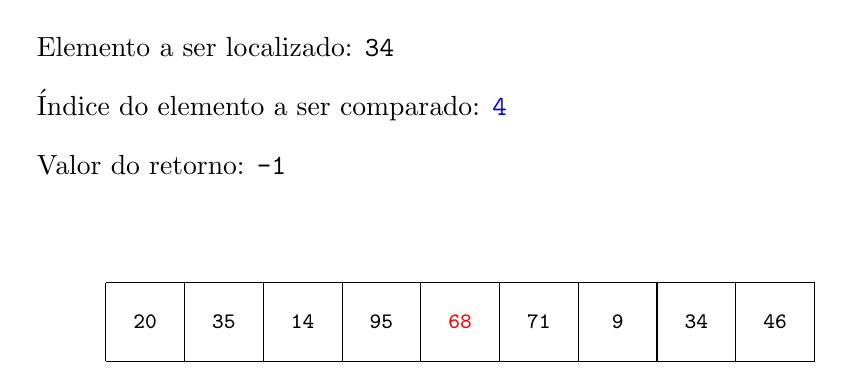
\begin{tikzpicture}
        \node[anchor=west] at (0, 4) {Elemento a ser localizado: \texttt{34}};
        \node[anchor=west] at (0, 3.25) {Índice do elemento a ser comparado: \texttt{\textcolor{blue}{4}}};
        \node[anchor=west] at (0, 2.5) {Valor do retorno: \texttt{-1}};
        \draw (1,0) grid (10,1);

        \node at (1.5,0.5) {\footnotesize \texttt{\textcolor{black}{20}}};
        \node at (2.5,0.5) {\footnotesize \texttt{\textcolor{black}{35}}};
        \node at (3.5,0.5) {\footnotesize \texttt{\textcolor{black}{14}}};
        \node at (4.5,0.5) {\footnotesize \texttt{\textcolor{black}{95}}};
        \node at (5.5,0.5) {\footnotesize \texttt{\textcolor{red}{68}}};
        \node at (6.5,0.5) {\footnotesize \texttt{71}};
        \node at (7.5,0.5) {\footnotesize \texttt{9}};
        \node at (8.5,0.5) {\footnotesize \texttt{34}};
        \node at (9.5,0.5) {\footnotesize \texttt{46}};
    \end{tikzpicture}

\end{frame}

\begin{frame}[fragile]{Exemplo de busca sequencial}

    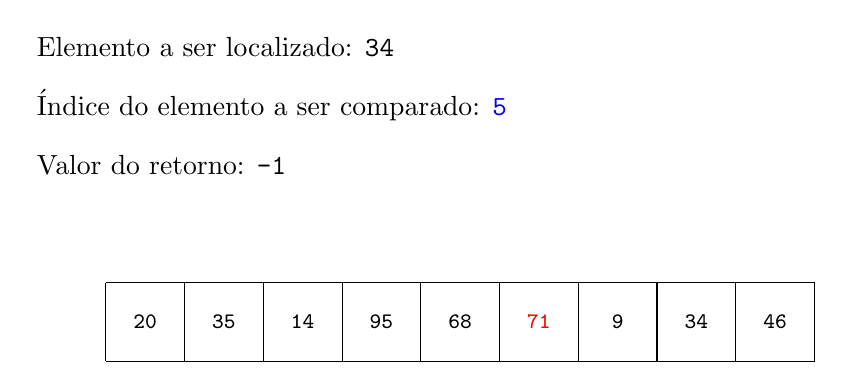
\begin{tikzpicture}
        \node[anchor=west] at (0, 4) {Elemento a ser localizado: \texttt{34}};
        \node[anchor=west] at (0, 3.25) {Índice do elemento a ser comparado: \texttt{\textcolor{blue}{5}}};
        \node[anchor=west] at (0, 2.5) {Valor do retorno: \texttt{-1}};
        \draw (1,0) grid (10,1);

        \node at (1.5,0.5) {\footnotesize \texttt{\textcolor{black}{20}}};
        \node at (2.5,0.5) {\footnotesize \texttt{\textcolor{black}{35}}};
        \node at (3.5,0.5) {\footnotesize \texttt{\textcolor{black}{14}}};
        \node at (4.5,0.5) {\footnotesize \texttt{\textcolor{black}{95}}};
        \node at (5.5,0.5) {\footnotesize \texttt{\textcolor{black}{68}}};
        \node at (6.5,0.5) {\footnotesize \texttt{\textcolor{red}{71}}};
        \node at (7.5,0.5) {\footnotesize \texttt{9}};
        \node at (8.5,0.5) {\footnotesize \texttt{34}};
        \node at (9.5,0.5) {\footnotesize \texttt{46}};
    \end{tikzpicture}

\end{frame}

\begin{frame}[fragile]{Exemplo de busca sequencial}

    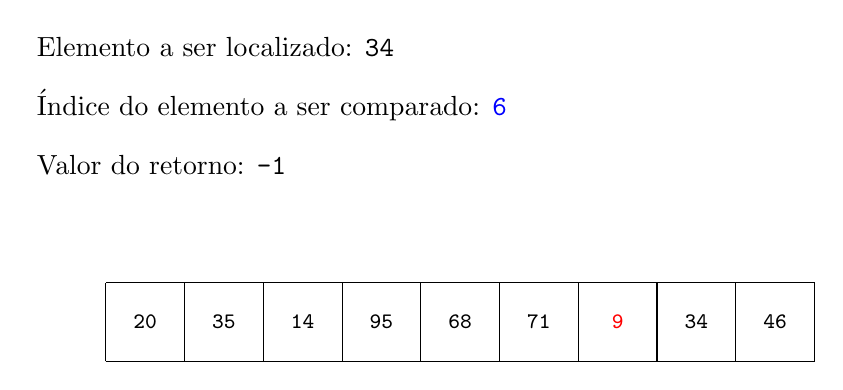
\begin{tikzpicture}
        \node[anchor=west] at (0, 4) {Elemento a ser localizado: \texttt{34}};
        \node[anchor=west] at (0, 3.25) {Índice do elemento a ser comparado: \texttt{\textcolor{blue}{6}}};
        \node[anchor=west] at (0, 2.5) {Valor do retorno: \texttt{-1}};
        \draw (1,0) grid (10,1);

        \node at (1.5,0.5) {\footnotesize \texttt{\textcolor{black}{20}}};
        \node at (2.5,0.5) {\footnotesize \texttt{\textcolor{black}{35}}};
        \node at (3.5,0.5) {\footnotesize \texttt{\textcolor{black}{14}}};
        \node at (4.5,0.5) {\footnotesize \texttt{\textcolor{black}{95}}};
        \node at (5.5,0.5) {\footnotesize \texttt{\textcolor{black}{68}}};
        \node at (6.5,0.5) {\footnotesize \texttt{\textcolor{black}{71}}};
        \node at (7.5,0.5) {\footnotesize \texttt{\textcolor{red}{9}}};
        \node at (8.5,0.5) {\footnotesize \texttt{34}};
        \node at (9.5,0.5) {\footnotesize \texttt{46}};
    \end{tikzpicture}

\end{frame}

\begin{frame}[fragile]{Exemplo de busca sequencial}

    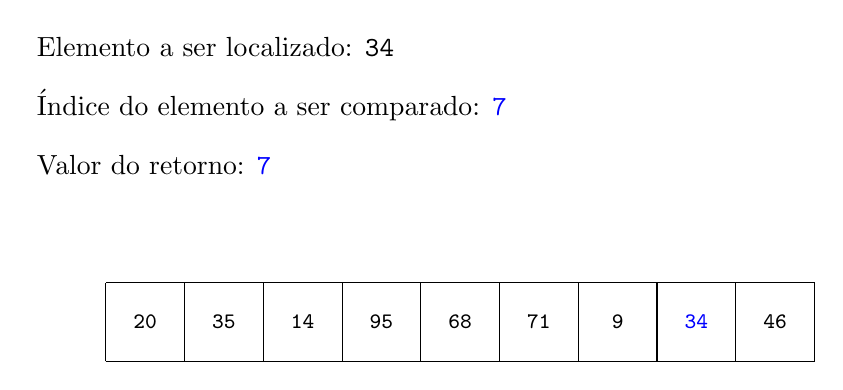
\begin{tikzpicture}
        \node[anchor=west] at (0, 4) {Elemento a ser localizado: \texttt{34}};
        \node[anchor=west] at (0, 3.25) {Índice do elemento a ser comparado: \texttt{\textcolor{blue}{7}}};
        \node[anchor=west] at (0, 2.5) {Valor do retorno: \texttt{\textcolor{blue}{7}}};
        \draw (1,0) grid (10,1);

        \node at (1.5,0.5) {\footnotesize \texttt{\textcolor{black}{20}}};
        \node at (2.5,0.5) {\footnotesize \texttt{\textcolor{black}{35}}};
        \node at (3.5,0.5) {\footnotesize \texttt{\textcolor{black}{14}}};
        \node at (4.5,0.5) {\footnotesize \texttt{\textcolor{black}{95}}};
        \node at (5.5,0.5) {\footnotesize \texttt{\textcolor{black}{68}}};
        \node at (6.5,0.5) {\footnotesize \texttt{\textcolor{black}{71}}};
        \node at (7.5,0.5) {\footnotesize \texttt{\textcolor{black}{9}}};
        \node at (8.5,0.5) {\footnotesize \texttt{\textcolor{blue}{34}}};
        \node at (9.5,0.5) {\footnotesize \texttt{46}};
    \end{tikzpicture}

\end{frame}

\begin{frame}[fragile]{Exemplo de uso de buca sequencial}
    \inputsnippet{c}{1}{21}{quadrinhos.c}
\end{frame}

\begin{frame}[fragile]{Exemplo de uso de buca sequencial}
    \inputsnippet{c}{23}{43}{quadrinhos.c}
\end{frame}

\begin{frame}[fragile]{Busca sequencial em C++}

    \begin{itemize}
        \item A biblioteca \code{c++}{algorithm} do C++ contém uma implementação da busca
            sequencial

        \item A função \code{c++}{find()} recebe dois iteradores $a$ e $b$, e um valor $x$, a
            ser procurado

        \item Caso $x$ se encontre dentre os elementos que estão no intervalo $[a, b)$, é
            retornado um iterador para a primeira ocorrência de $x$

        \item Caso $x$ não esteja no intervalo, é retornado o valor $b$

        \item A sintaxe da função \code{c++}{find()} é
            \inputsyntax{c++}{find.st}

        \item Esta função pode ser usada em qualquer contêiner que tenha iteradores que suportem
            a operação de incremento e que armazenem qualquer tipo que suporte o operador de
            comparação \code{c++}{==}
    \end{itemize}

\end{frame}

\begin{frame}[fragile]{Exemplo de uso da função \code{c++}{find()}}
    \inputcode{c++}{find.cpp}
\end{frame}

\begin{frame}[fragile]{Travessias e Filtros}

    \begin{itemize}
        \item O processo de se visitar cada um dos elementos contidos em um contêiner é
            denominado travessia

        \item A busca sequencial usa uma travessia para confrontar cada um dos elementos 
            do contêiner contra o valor que se deseja localizar

        \item Um padrão comum associado à travessia é o de se escolher um ou mais elementos do
            contêiner, de acordo com um predicato $P$

        \item Um predicato $P$ é uma função que recebe, dentre seus parâmetros, um elemento $e$ do 
        tipo $T$ e retorna ou verdadeiro ou falso

        \item Este padrão recebe o nome de filtro

        \item Uma busca sequencial é um filtro que seleciona um (ou mais) elemento do contêiner
            com o predicado $P$ definido como
            \inputsyntax{c++}{P.cpp}

    \end{itemize}

\end{frame}

\begin{frame}[fragile]{Filtros em C++}

    \begin{itemize}
        \item A biblioteca \code{c++}{algorithm} do C++ contém uma implementação genérica de
            filtros

        \item A função \code{c++}{copy_if()} recebe um par de iteradores $a$ e $b$, que 
            definem um intervalo $[a, b)$; um iterador de saída $s$, onde serão escritos
            os elementos que atendem o filtro; e um predicato $P$ unário (que aceita um único
            parâmetro do tipo $T$)

        \item Todos os elementos $e$ tais que $P(e)$ é verdadeiro serão copiados no iterador de
            saída $s$

        \item A sintaxe da função \code{c++}{copy_if()} é 
            \inputsyntax{c++}{copy_if.st}

        \item A função \code{c++}{back_inserter()}, da biblioteca \code{c++}{iterator}, gera
            um iterador de saída para o contêiner passado como parâmetro

        \item O contêiner em questão deve ter suporte para a função \code{c++}{push_back()}

    \end{itemize}

\end{frame}

\begin{frame}[fragile]{Exemplo de uso de filtro}
    \inputcode{c++}{bs.cpp}
\end{frame}

\begin{frame}[fragile]{Transformações}

    \begin{itemize}
        \item Outro padrão associado à travessia é a transformação

        \item Uma transformação visita cada um dos elementos $x$ de $S$, e o substitui pelo 
            resultado da transformação $T(x)$

        \item A bilioteca \code{c++}{algorithm} do C++ implementa transformações através da
            função \code{c++}{transform()}

        \item A sintaxe da função \code{c++}{transform()} é
            \inputsyntax{c++}{transform.st}

        \item Há também uma versão da função \code{c++}{transform()} que aceita uma operação
            binária
    \end{itemize}

\end{frame}

\begin{frame}[fragile]{Exemplo de uso de transformações}
    \inputcode{c++}{dot.cpp}
\end{frame}
